\section{Обзор методов оценки RAG-систем}
\label{sec:related_work}

В данном разделе рассматриваются современные подходы, фреймворки и
модели, применяемые для автоматической оценки RAG-систем. Цель раздела —
показать, на каких методологических принципах
основан предлагаемый в настоящей работе подход, а также обосновать выбор
RAGBench/TRACe в качестве основы для русскоязычной адаптации.

\subsection{RAGAS}
\label{sec:ragas}

RAGAS (Retrieval Augmented Generation Assessment)~\cite{es2024ragas} - один из
 первых автоматических фреймворков оценки RAG. Он использует LLM (в оригинале - GPT-3.5/4) 
 для вычисления трёх метрик: \emph{Faithfulness} (достоверность ответа относительно контекста),
  \emph{Answer Relevance} (релевантность ответа вопросу) и \emph{Context Relevance} 
  (релевантность извлечённого контекста вопросу).

\textbf{Faithfulness.} Ответ $A$ разбивается LLM на атомарные утверждения
 $S = \{s_1, \dots, s_n\}$; для каждого $s_i$ новым запросом проверяется, поддерживается
  ли оно текстом контекста $c(q)$. Метрика:
\[
F = \frac{|V|}{|S|},\quad |V| = \sum_{i=1}^{|S|} v\bigl(s_i, c(q)\bigr).
\]

\textbf{Answer Relevance.} Из ответа $A$ генерируется набор 
вопросов $\{q_i\}_{i=1}^n$, и считается средняя косинусная близость между
 исходным вопросом $q$ и каждым $q_i$ в пространстве \glslink{эмбеддинг}{эмбеддингов}:
\[
AR = \frac{1}{n}\sum_{i=1}^{n}\cos\bigl(\phi(q), \phi(q_i)\bigr).
\]

\textbf{Context Relevance.} LLM извлекает из контекста подмножество 
релевантных предложений $S_\text{ext}$; метрика - отношение $|S_\text{ext}| / |\text{sentences}(c(q))|$.

\noindent\textbf{Преимущества.} RAGAS не требует ручной разметки эталонных 
оценок, имеет модульную структуру и поддерживает интеграцию с различными 
LLM, эмбеддинговыми моделями и ретриверами. Благодаря этому фреймворк может 
быть адаптирован к разным доменам и языкам при наличии подходящих моделей 
для генерации, оценки и построения эмбеддингов.

\noindent\textbf{Ограничения.} Основные ограничения RAGAS связаны с зависимостью 
значительной части метрик от внешнего LLM-оценщика, что повышает стоимость 
вычислений и может снижать воспроизводимость результатов при изменении модели, 
промпта или параметров генерации. Для русского языка применение RAGAS требует 
использования мультиязычных или русскоязычных LLM и эмбеддинговых моделей; 
при этом отсутствует общепринятая русскоязычная валидационная разметка, 
позволяющая независимо оценить надёжность получаемых метрик.

\subsection{RAGBench и фреймворк TRACe}
\label{sec:ragbench}

RAGBench~\cite{friel2024ragbench} - масштабный бенчмарк из 100~тыс. 
примеров в 12 поддатасетах, покрывающих пять доменов: биомедицина (PubMedQA, CovidQA),
 общие знания (HotpotQA, MS~Marco, HAGRID, ExpertQA), юридические контракты (CuAD),
  клиентская поддержка (DelucionQA, EManual, TechQA) и финансы (FinQA, TAT-QA). 
  Каждый пример размечен четырьмя метриками фреймворка TRACe:

\textbf{1. Relevance.} Доля релевантных токенов в документах контекста относительно общего числа:
\[
\text{relevance} = \frac{\sum_{i} |R_i|}{\sum_{i} |d_i|},
\]
где $R_i$ - множество релевантных токенов документа $d_i$.

\textbf{2. Utilization.} Доля использованных в ответе токенов контекста:
\[
\text{utilization} = \frac{\sum_{i} |U_i|}{\sum_{i} |d_i|}.
\]

\textbf{3. Completeness.} Доля релевантных токенов, которые реально были использованы:
\[
\text{completeness} = \frac{\sum_{i} |R_i \cap U_i|}{\sum_{i} |R_i|}.
\]

\textbf{4. Adherence.} Булева метрика: все ли утверждения в ответе подтверждаются контекстом.
 Позволяет обнаруживать галлюцинации.

Разметка формируется с использованием LLM-аннотатора на основе GPT-4: для каждого 
примера модель выделяет релевантные предложения в документах, определяет фрагменты, 
использованные при формировании ответа, а также проверяет, подтверждается ли каждое 
предложение ответа предоставленным контекстом. Валидация на синтетических данных KILT с
 известными эталонными оценками показала высокую ранговую корреляцию по коэффициенту 
 Кендалла \cite{kendall1938new}, что авторы рассматривают как подтверждение надёжности 
 автоматической разметки.

Важной методологической особенностью RAGBench является
 сравнение различных оценщиков на одном и том же наборе данных
 (рис.~\ref{benchmark:image1}). Согласно результатам авторов оригинальной
 статьи~\cite{friel2024ragbench}, дообученная DeBERTa-v3-large предсказывает
 TRACe-метрики на англоязычных поддатасетах точнее, чем большая языковая
 модель без дообучения~\cite{brown2020language} в схожем формате запроса,
 а также фреймворки RAGAS и TruLens. Это наблюдение относится к работе авторов
 RAGBench и в настоящей диссертации напрямую не воспроизводится; оно
 рассматривается как методологический ориентир, обосновывающий направление,
 при котором локальная специализированная модель может выступать более дешёвой
 заменой вызовам большой языковой модели.

\begin{figure}[H]
    \centering
    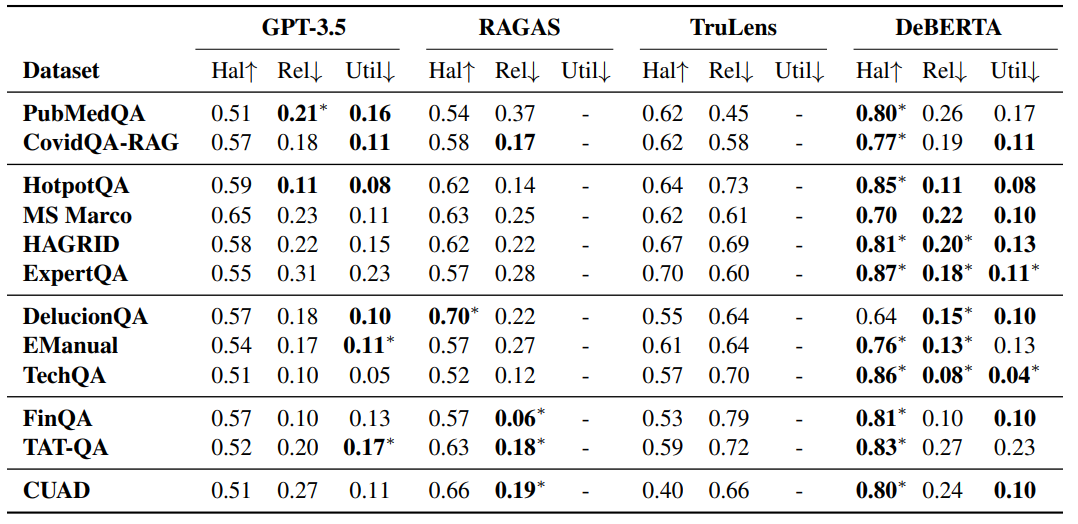
\includegraphics[width=0.8\textwidth]{table1.png}
    \caption{Сравнение методов оценки на тестовых сплитах RAGBench \cite{friel2024ragbench}}
    \label{benchmark:image1}
\end{figure}

\noindent\textbf{Преимущества.} RAGBench представляет собой масштабный
и доменно -  диверсифицированный корпус, содержащий интерпретируемый набор
токен-уровневых метрик. Дополнительным преимуществом является демонстрация 
того, что дообучение специализированного оценщика позволяет существенно 
повысить качество автоматической оценки по сравнению с zero-shot подходами.

\noindent\textbf{Ограничения.} Основными ограничениями RAGBench являются 
ориентация на английский язык, отсутствие отдельных метрик отказа от ответа 
и безопасности, а также зависимость качества разметки от LLM-аннотатора 
на основе GPT-4.

\subsection{Luna}
\label{sec:luna}

Luna~\cite{belyi2024luna} — специализированный оценщик
галлюцинаций в RAG-системах, предназначенный для промышленного применения.
Модель основана на энкодере DeBERTa-v3-Large с 440 млн параметров,
дообученном определять, какие токены ответа подтверждаются
переданным контекстом.  В качестве начальной
точки используется версия модели, предварительно обученная на задаче вывода
на естественном языке (Natural Language Inference, NLI), где требуется
определять отношение между двумя текстами: логическое следование, противоречие
или нейтральность. Голова предсказания инициализируется весами
NLI-классификатора, что позволяет перенести эту постановку на задачу
токен-уровневой проверки ответа по контексту.

Для обработки длинного контекста вход разбивается на окна длиной $L$, каждое 
из которых содержит часть контекста, вопрос и полный ответ:
\[
w_i = [c_{i_1}\ldots c_{i_l}] \oplus [q_1\ldots q_Q] \oplus [r_1\ldots r_R],
\]
где $l = L - Q - R$. Для каждого окна модель предсказывает вероятности поддержки 
токенов ответа:
\[
P_S(w_i) = [p^i_1,\ldots,p^i_R].
\]
На этапе инференса для каждого токена ответа выбирается максимальная вероятность 
поддержки среди всех окон:
\[
p_j = \max_i p^i_j,
\]
после чего вероятность поддержки всего ответа определяется как минимальная 
вероятность среди токенов:
\[
P_S = \min_j p_j,\quad P_H = 1 - P_S,
\]
где $P_H$ трактуется как вероятность галлюцинации ответа.

Экспериментальные результаты показывают, что Luna превосходит оценщики 
на базе GPT-3.5, а также фреймворки RAGAS и TruLens, в задаче обнаружения 
галлюцинаций при существенно меньших вычислительных затратах и меньшем времени 
получения оценки. На наборе RAGTruth модель показывает более высокое качество 
по сравнению с подходами, основанными на прямых запросах к большим языковым 
моделям, в задачах вопросно-ответной генерации и автоматического резюмирования. 
На внутреннем тестовом наборе RAG QA Luna также превосходит рассмотренные 
базовые оценщики во всех предметных направлениях. Таким образом, Luna 
демонстрирует практическую применимость подхода, при котором специализированная 
локальная модель может выступать менее затратной и более быстрой альтернативой 
оценщику на основе большой языковой модели.

Отдельно следует отметить связь Luna с RAGBench/TRACe. Хотя в статье, 
посвящённой RAGBench, явная ссылка на Luna отсутствует, в личной переписке с авторами RAGBench было уточнено, что при построении 
RAGBench использовались отдельные инженерные решения, близкие к Luna, включая 
оконное разбиение длинного контекста и аугментации документов. В связи с этим 
Luna представляет интерес не только как самостоятельный оценщик галлюцинаций, 
но и как пример инженерной реализации подходов, применимых при построении 
специализированного локального оценщика RAG-систем.

\subsection{ARES}
\label{sec:ares}

ARES~\cite{saad2023ares} предлагает автоматизированный подход к оценке
RAG-систем, основанный на обучении специализированных моделей-оценщиков
на синтетических данных. В качестве основных критериев 
рассматриваются релевантность найденного контекста запросу, обоснованность 
ответа предоставленным контекстом и релевантность ответа исходному вопросу. 
На первом этапе большая языковая модель генерирует синтетические тройки 
<<запрос -- фрагмент контекста -- ответ>>, включающие как положительные, 
так и отрицательные примеры. Отрицательные примеры формируются не только 
за счёт некорректных или противоречивых ответов, но и за счёт нерелевантных 
фрагментов контекста и ответов, не соответствующих исходному запросу. 
Затем на этих данных дообучаются отдельные модели-оценщики для каждого 
из рассматриваемых критериев, например на основе DeBERTa-v3-Large.

Важной особенностью ARES является сочетание синтетического обучения 
с небольшим объёмом ручной разметки: для повышения надёжности итоговой 
оценки авторы используют набор человеческих аннотаций и метод 
prediction-powered inference, позволяющий корректировать ошибки 
модели-оценщика и строить доверительные интервалы для сравнения RAG-систем. 
Тем самым ARES не полностью исключает ручную разметку, но существенно 
снижает её необходимый объём.

Преимуществом ARES является возможность получать специализированные 
оценщики для конкретного домена без формирования крупного вручную 
размеченного корпуса. Ограничение подхода связано с тем, что качество 
обучаемого оценщика зависит от распределения и качества синтетически 
сгенерированных примеров, а также от репрезентативности небольшого 
валидационного набора с ручной разметкой.

В контексте настоящей работы идея ARES используется частично: большая
языковая модель Qwen2.5-72B применяется для перевода исходного корпуса
и в качестве zero-shot LLM-оценщика для сравнения, однако не выступает
в качестве финального оценщика. Финальная оценка, как и в направлении
ARES/RAGBench, переносится на специализированную локальную модель, что
позволяет снизить стоимость и повысить воспроизводимость автоматической оценки.

\subsection{RAGTruth}
\label{sec:ragtruth}

RAGTruth~\cite{niu2023ragtruth} - корпус почти из 18~тыс. ответов, 
сгенерированных RAG-системами и вручную размеченных для задачи обнаружения 
галлюцинаций. Разметка выполнена как на уровне всего ответа, так и на уровне 
отдельных слов, что позволяет выделять неподтверждённые или противоречащие 
контексту фрагменты. 

Сильной стороной RAGTruth является высокое качество ручной разметки и более 
детальный анализ галлюцинаций по сравнению с оценкой только на уровне всего 
ответа. Вместе с тем корпус не содержит разметки в схеме TRACe: в нём отсутствуют 
отдельные токен-уровневые метки релевантности контекста и использования 
контекста в ответе. Поэтому в настоящей работе RAGTruth не используется как 
обучающий корпус, однако служит полезным ориентиром при анализе ошибок 
LLM-оценщика.

\subsection{AttributionBench}
\label{sec:attribution}

AttributionBench~\cite{li2024attributionbench} фокусируется на задаче 
автоматической оценки атрибуции ответа источнику, то есть проверки того, 
подтверждается ли каждое утверждение в сгенерированном ответе приведённым 
доказательством. Авторы показывают, что эта задача остаётся сложной даже 
для современных больших языковых моделей: качество GPT-4 и GPT-3.5 заметно 
зависит от постановки запроса, а простое изменение промпта не решает проблему 
надёжной оценки.

Основной вывод работы состоит в том, что атрибуцию ответа к источнику трудно 
надёжно оценивать одним запросом к LLM без дополнительной настройки. Это 
поддерживает общий вывод настоящей работы о необходимости специализированных 
оценщиков, в том числе моделей, обучаемых для проверки связи между контекстом 
и отдельными фрагментами ответа.

\subsection{Сравнение фреймворков}

Сводная характеристика рассмотренных фреймворков приведена в таблице~\ref{tab:frameworks}. 
Для настоящей работы RAGBench/TRACe выбран в качестве базы по совокупности признаков: 
наличие публично доступного корпуса достаточного объёма, интерпретируемые метрики на уровне 
токенов, эмпирически обоснованная стратегия обучения компактного оценщика, и возможность 
использовать LLM-аннотатор только на этапе разметки (а не во время применения).

\begin{table}[H]
\centering
\footnotesize
\caption{Сравнение рассмотренных подходов к оценке RAG-систем}
\label{tab:frameworks}
\resizebox{\textwidth}{!}{%
\begin{tabular}{lccccc}
\toprule
Подход / ресурс & Тип оценки & Разметка & Уровень детализации & Открытый корпус & Язык \\
\midrule
RAGAS~\cite{es2024ragas}   
& LLM-оценщик        
& не требуется         
& уровень ответа / контекста  
& нет 
& EN / мультиязычный \\

ARES~\cite{saad2023ares}   
& обучаемый оценщик        
& синтетическая + малая ручная   
& уровень примера  
& нет 
& EN \\

RAGTruth~\cite{niu2023ragtruth} 
& корпус для анализа галлюцинаций      
& ручная      
& уровень ответа и слов 
& да 
& EN \\

AttributionBench~\cite{li2024attributionbench} 
& корпус для оценки атрибуции 
& ручная 
& уровень утверждений 
& да 
& EN \\

Luna~\cite{belyi2024luna}  
& обучаемый оценщик        
& NLI + RAG-данные   
& уровень токенов ответа 
& частично 
& EN \\

RAGBench~\cite{friel2024ragbench} 
& обучаемый оценщик + LLM-аннотатор 
& GPT-4 
& уровень токенов 
& да 
& EN \\

\textbf{RAGBench-RU (настоящая работа)}
& обучаемый оценщик + zero-shot LLM-оценщик
& перенос исходной разметки RAGBench после перевода
& уровень токенов
& да
& \textbf{RU} \\
\bottomrule
\end{tabular}%
}
\end{table}

\noindent\textbf{Вывод.} Проведённое сравнение показывает, что существующие 
подходы решают разные аспекты задачи оценки RAG-систем. RAGAS удобен как 
готовый инструмент без необходимости предварительной разметки, ARES показывает 
возможность обучения оценщиков на синтетических данных, RAGTruth и 
AttributionBench дают качественные ручные корпуса для анализа галлюцинаций 
и атрибуции, а Luna демонстрирует практическую эффективность локального 
обучаемого оценщика.

При этом наиболее подходящей отправной точкой для настоящей работы является 
RAGBench/TRACe, поскольку он сочетает открытый корпус, интерпретируемую 
токен-уровневую схему разметки и возможность перенести финальную оценку 
с большой языковой модели на специализированный локальный классификатор. 
Именно это делает RAGBench/TRACe удобной основой для русскоязычной адаптации. 
В следующем разделе формализуется задача, решаемая в настоящей работе.
